\section{AI-Assisted Schema Generation Design}
\label{sec:schema_gen_design}

The previous section described schema generation from the backend's point of view: the Go API forwards a natural-language request to an external service, caches the returned DDL under a project-scoped key, and applies it only after the user approves. This section looks inside that external service and explains how it is designed. The theoretical grounding for the techniques used here (multi-agent LLM systems, tool use, and retrieval-augmented generation) was already covered in Section~\ref{ch2:sec4}, so the focus below is on the concrete design decisions rather than the underlying theory.

The service takes a plain-language description of an application and produces a relational design for it: an entity-relationship view, a normalized set of tables in third normal form, executable PostgreSQL DDL, and a human-readable report. The hard part is not generating SQL text; a single prompt can do that. The hard part is producing a design that is internally consistent, correctly keyed, normalized, and faithful to the requirement. The design therefore treats schema generation as a small engineering workflow rather than a single model call. Figure~\ref{fig:schema_arch} gives the overall architecture, and the subsections that follow explain each part.

\begin{figure}[H]
    \centering
    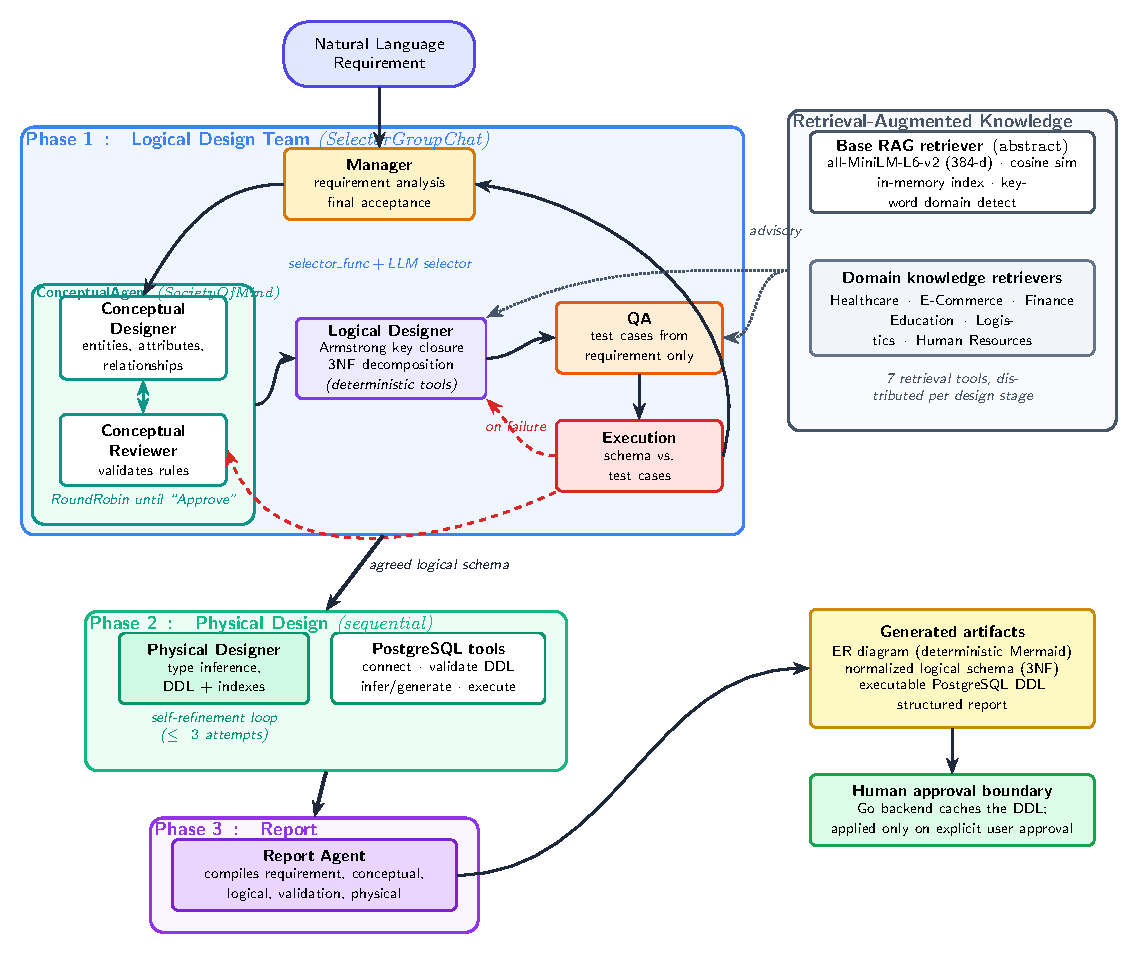
\includegraphics[width=\linewidth,height=0.9\textheight,keepaspectratio]{images/ai/schema_architecture.pdf}
    \caption{Multi-agent schema generation architecture.}
    \label{fig:schema_arch}
\end{figure}

\subsection{Design Goals}

The service was shaped by five goals that often pull against each other:

\begin{itemize}
    \item \textbf{Correctness over fluency.} A schema that reads well but loses a foreign key or violates normalization is worse than useless. Key discovery and normalization are treated as steps that must be verifiable, not left to free generation.
    \item \textbf{Human in the loop.} The service proposes; it never commits. Generated DDL is reviewed and approved by the user through the backend before it ever touches a tenant database.
    \item \textbf{Domain awareness.} A hospital schema and an online store schema follow different conventions. The design lets curated domain knowledge steer the model toward sensible entities, relationships, and types.
    \item \textbf{Model independence.} The workflow should not be tied to one model vendor, so the choice of large language model is a runtime parameter rather than a structural assumption.
    \item \textbf{Visible progress.} Generation can take time, so the design exposes intermediate work as it happens instead of leaving the user waiting on a blank screen.
\end{itemize}

\subsection{Decomposition into Specialized Agents}

Rather than ask one model to do everything, the service splits the work across agents that each own one stage of the classical database design lifecycle. This mirrors how a human team would approach the same task and, more importantly, it lets each stage be checked before the next one builds on it. Table~\ref{tab:schema_agents} lists the roles, and Figure~\ref{fig:schema_arch} shows how they are wired together.

\begin{table}[H]
    \centering
    \small
    \renewcommand{\arraystretch}{1.3}
    \begin{tabularx}{\textwidth}{|>{\RaggedRight\arraybackslash}p{3.4cm}|>{\RaggedRight\arraybackslash}X|}
    \hline
    \textbf{Agent} & \textbf{Responsibility} \\
    \hline
    Manager & Reads the requirement, fills in implied but unstated needs, and later decides final acceptance. \\
    \hline
    Conceptual Designer & Extracts entity sets, attributes, relationships, and cardinalities into a structured entity-relationship model. \\
    \hline
    Conceptual Reviewer & Checks the conceptual model against design rules (every entity participates in a relationship, relationship attributes carry no identifiers, valid cardinalities) and asks for revisions. \\
    \hline
    Logical Designer & Converts the approved conceptual model into normalized relations with primary and foreign keys, using deterministic tools for key discovery and third-normal-form decomposition. \\
    \hline
    QA & Generates representative insert, update, query, and delete cases from the requirement, without seeing the schema, to test it independently. \\
    \hline
    Execution & Judges whether the proposed schema satisfies those cases and routes failures back to the responsible designer. \\
    \hline
    Physical Designer & Infers concrete PostgreSQL types, writes executable DDL with indexes, and validates it against a real database. \\
    \hline
    Report & Compiles the requirement, conceptual, logical, validation, and physical results into one structured document. \\
    \hline
    \end{tabularx}
    \caption{Agent roles in the schema generation service.}
    \label{tab:schema_agents}
\end{table}

A deliberate design choice is that the conceptual, logical, and validation agents work together as a coordinated group, while the physical designer runs afterward as a separate step. The reason is that physical design only consumes the agreed logical model; it does not contribute opinions back into the design debate. Keeping it outside the group avoids letting low-level type and index decisions pollute the higher-level discussion about entities and relationships.

\subsection{Coordination and Feedback Loops}

Two feedback loops give the workflow its self-correcting behavior.

The first is an inner loop around conceptual design. The conceptual designer and the reviewer exchange turns until the reviewer is satisfied and signals approval. The reviewer applies a fixed validation procedure rather than a vague judgment, so its objections are concrete and the designer knows exactly what to fix. This whole exchange is packaged so that the rest of the workflow sees only one agreed conceptual model, not the back-and-forth that produced it.

The second is an outer validation loop. After the QA agent writes test cases and the execution agent evaluates the schema against them, a failure is not fatal. The execution agent routes the problem back to whichever stage caused it: a missing or wrong entity sends the work back to conceptual design, while a keying or normalization mistake sends it back to logical design. Once corrected, the work flows forward again through validation. Both loops are bounded by a maximum number of exchanges so the service cannot loop forever on a requirement it cannot satisfy; if the bound is reached, the best current design is returned rather than nothing.

This structure is what turns a collection of prompts into a process. Errors are caught close to where they are introduced, which keeps a single early mistake from cascading into a broken final schema.

\subsection{Domain-Aware Retrieval Design}

General models know a little about every domain and a lot about none. To raise the quality of designs in common application areas, the service is paired with a curated knowledge base that the agents can consult while they work. This is a retrieval-augmented design, but with an important twist: the knowledge is ground truth that is authored and version-controlled as part of the system, not scraped from open sources at query time. That keeps the guidance consistent, reviewable, and free of the noise and licensing concerns of open retrieval.

When a requirement arrives, the service infers its domain from the language used and, if a matching knowledge base exists, makes that knowledge available to the agents. Retrieval is targeted to each stage: the conceptual designer and reviewer ask for standard entities and relationship patterns, the logical designer asks for cardinality and normalization guidance, and the physical designer asks for type mappings. If no domain is recognized, the agents fall back to general database design principles and the workflow proceeds unchanged.

The knowledge base spans six application domains, summarized in Table~\ref{tab:rag_domains}. Each domain encodes the entities that typically appear, the relationships among them, the cardinality and normalization conventions that apply, and the data types that suit its attributes. Sensitive domains also carry handling flags so that fields representing protected or personal information can be marked as such during design.

\begin{table}[H]
    \centering
    \small
    \renewcommand{\arraystretch}{1.3}
    \begin{tabularx}{\textwidth}{|>{\RaggedRight\arraybackslash}p{3.2cm}|>{\RaggedRight\arraybackslash}X|}
    \hline
    \textbf{Domain} & \textbf{Representative knowledge} \\
    \hline
    Healthcare & Patients, providers, encounters, diagnoses, medications, observations, appointments, insurance, and the clinical relationships among them; flags for protected health information. \\
    \hline
    E-Commerce & Customers, products and variants, categories, carts, orders and line items, payments, inventory, reviews, and discounts. \\
    \hline
    Finance and Banking & Accounts, customers, transactions, ledgers, cards, loans, branches, and statements, with conventions for monetary and audit fields. \\
    \hline
    Education and Academia & Students, instructors, courses, sections, enrollments, departments, terms, and grading structures. \\
    \hline
    Logistics and Supply Chain & Shipments, warehouses, carriers, routes, suppliers, purchase orders, inventory, and tracking events. \\
    \hline
    Human Resources & Employees, departments, positions, payroll, attendance, leave requests, benefits, and performance reviews, with flags for personal data. \\
    \hline
    \end{tabularx}
    \caption{Application domains covered by the curated knowledge base.}
    \label{tab:rag_domains}
\end{table}

Retrieval is advisory, not binding. The agents are free to adapt or ignore the guidance when the requirement calls for something the standard pattern does not cover. The aim is to give the model a strong, opinionated starting point in familiar territory while keeping it general enough to handle anything else.

\subsection{Outputs and the Approval Boundary}

The service emits four artifacts: an entity-relationship diagram, a normalized logical schema as structured data, executable PostgreSQL DDL with indexes, and a report that ties the pieces together with the reasoning behind them. None of these are applied automatically. As described in the previous section, the backend caches the proposed DDL and waits for explicit user approval before running it against a tenant database. This boundary is a security design decision as much as a usability one: the AI service can suggest a schema, but only an authenticated, deliberate action by the project owner can change real data. The model never holds a connection to a tenant database, so there is no path by which a generated statement can mutate data on its own.
